\documentclass[border=3pt]{standalone}

% Drawing
\usepackage{tikz}

% Tikz Library
\usetikzlibrary{3d, shapes.multipart}

% Styles
\tikzset{>=latex} % for LaTeX arrow head
\tikzset{axis/.style={black, thick,->}}
\tikzset{vector/.style={>=stealth,->}}
\tikzset{every text node part/.style={align=center}}

% Newcommand
%% Viewing Screen
\newcommand{\rect}[1]{%
	\begin{scope}[canvas is xz plane at y=1.2]
		\draw[thick, fill=black!40] (#1,-1.2) rectangle (#1+0.2,1.2);
	\end{scope}
	%
	\begin{scope}[canvas is xy plane at z=1.2]
		\draw[thick, fill=black!25](#1,-1.2) rectangle (#1+0.2,1.2);
	\end{scope}
	%
	\begin{scope}[canvas is yz plane at x=#1]
		\draw[thick, fill=black!10] (-1.2,-1.2) rectangle (1.2,1.2);
		\draw[thick, fill=black!10, dashed] (0,-0.65) -- (0,0.65);
	\end{scope}
}
%% Draw in Polar Coordinates from (0,0) to (r,theta)
\newcommand{\cdraw}[2]{\draw[very thick, -stealth, red] (0,0) -- ({#1*cos(#2)}, {#1*sin(#2)});}

% Notation
\usepackage{amsmath}

\begin{document}

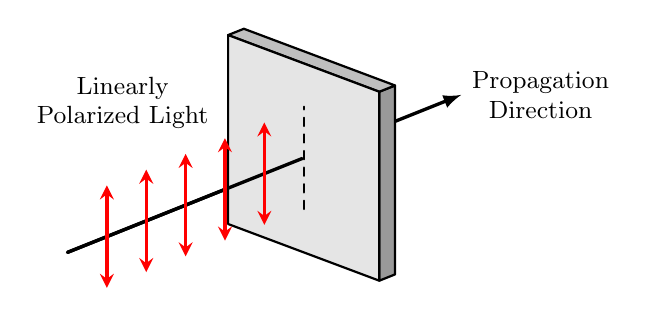
\begin{tikzpicture}[x={(1cm,0.4cm)}, y={(8mm, -3mm)}, z={(0cm,1cm)}, line cap=round, line join=round]
	
	% Main Axes
%	\draw[->] (0,0,0) -- (6,0,0) node[right] {$x$};
%	\draw[->] (0,0,0) -- (0,2,0) node[below left] {$y$};
%	\draw[->] (0,0,0) -- (0,0,2) node[above] {$z$};
	
	% Propagation Axis
	\draw[very thick, ->] (1,0,0) -- (6,0,0) node[right, black] {\small{Propagation}\\[-0.5mm]\small{Direction}};
	
	% Viewing Screen
	\rect{4}
		
	% Correction for 3D 
	\draw[very thick] (1,0,0) -- (3.98,0,0);
	
	% Polarized Light (Red Arrows)
	\foreach \i in {1.5,2,...,3.5}
	{
		\begin{scope}[canvas is yz plane at x=\i]
		
			\cdraw{0.65}{90}
			\cdraw{0.65}{270}
			
		\end{scope}
	}
	
	% Node 
	\node at (2.5,-1,1) {\small{Linearly}\\[-0.5mm]\small{Polarized Light}};
\end{tikzpicture}

\end{document}
